\StartPlate{V08}{Two defining-sequence examples}{The recursion records levels and field refinements, not just its final matrix size.}
\begin{center}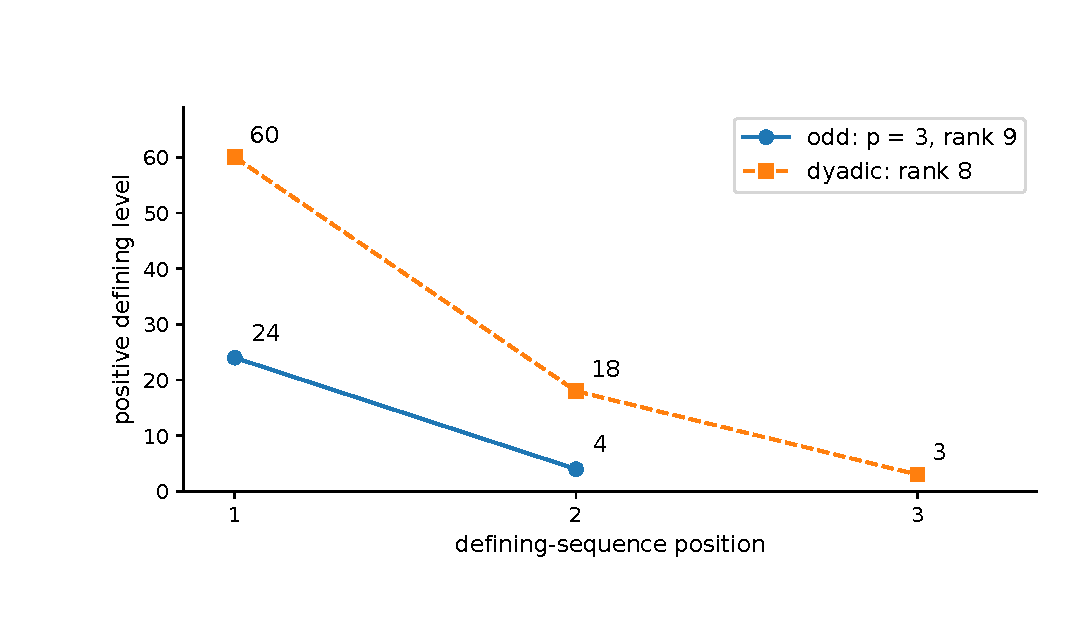
\includegraphics[width=\linewidth]{figures/V08.pdf}\end{center}
The odd example uses $p=3$, $d=2$, and $(h_1,h_2)=(1,2)$. Its displayed levels are $(24,4)$. The dyadic example uses $d=3$ and $(h_1,h_2,h_3)=(1,3,5)$, giving $(60,18,3)$. Each position refers to that example's own defining sequence.
\[
\nu_j=p^{d-j}(p+1)h_{d-j+1}
\quad\text{or}
\quad\nu_j=2^{d-j}3h_{d-j+1}.
\]
The two plotted lines are not empirical fits or samples of one common arithmetic family. They make the inherited level formulas legible. In the odd example, $24>3\cdot4>2\cdot4$ illustrates the separated scales used in refinement.

Supplying the levels does not prove that the literal corrected matrix generates the asserted maximal field. That conclusion uses the filtered corestriction lift and the precise refinement theorem. In the dyadic argument, separability from native trace one is established only after the full field degree has been obtained.
\vfill\PlateSource{Inherited formulas, exact evaluation}{Part I, Sections 7.1--7.4 and 8.1--8.3}{12}
